\documentclass[11pt,a4paper,oneside]{article}


\usepackage[utf8]{inputenc}
\usepackage{amsmath}
\usepackage{amsfonts}
\usepackage{amssymb}
\usepackage{graphicx}
\author{Igo Ramalho Brilhante \and Tales Parente}

\newcommand{\HRule}{\rule{\linewidth}{0.5mm}}

% BEFORE SUBMITTING FOR REVIEW, PLEASE:
% 1. Run a spell-checker:
% 2. Check anonymity constraints, if needed:
% 3. Change chato-notes to hide:
%\usepackage[showx]{style/chato-notes}
\usepackage[show]{../extras/chato-notes}



\newcounter{uc-counter} \setcounter{uc-counter}{1}
\newenvironment{uc}[1][]{\medskip\noindent \textbf{Caso de Uso \arabic{uc-counter}}}{\medskip \stepcounter{uc-counter}}

\begin{document}

\newcommand{\ucform}[8][]{
\begin{itemize}
	\item Identificador: \textbf{#2}\textbf{\arabic{uc-counter}}
	\item Nome: #3
	\item Descrição: #4
	\item Prioridade: #5
	\item Fluxo de eventos: #6
	\item Pré-condições e restrições: #7
	\item Pós-condições: #8
\end{itemize}
}

\begin{titlepage}
\begin{center}

% Upper part of the page. The '~' is needed because \\
% only works if a paragraph has started.

\includegraphics[scale=0.3]{../figuras/brasao_ufc.jpg}~\\[1cm]

\textsc{\LARGE Universidade Federal do Ceará}\\[1.5cm]

\textsc{\Large Recomenda AI - \textsc{RAI}}\\[0.5cm]

% Title
\HRule \\[0.4cm]
{ \huge \bfseries Documento de Requisitos}\\[0.4cm]

\HRule \\[1.5cm]

% Author and supervisor
\begin{minipage}{0.4\textwidth}
\begin{flushleft} \large
\emph{Equipe:}\\
Igo \textsc{Brilhante}\\
Tales \textsc{Parent}
\end{flushleft}
\end{minipage}
%\begin{minipage}{0.4\textwidth}
%\begin{flushright} \large
%\emph{Professores:} \\
%Dr.~Mark \textsc{Brown}
%\end{flushright}
%\end{minipage}

\vfill

% Bottom of the page
{\large Junho 2013}

\end{center}
\end{titlepage}

\section{Introdução}
\note{Introduzir o sistema, aplicação móvel e servidor}

Este documento tem como objetivo descrever os requisitos necessários para a elaboração do sistema \emph{Recomenda Ai - RAI}. Esse sistema é constituído de uma aplicação móvel e um servidor que fica na nuvem (Figura \ref{fig:arquitetura-rai}).

O objetivo do sistema é oferecer serviços de sugestões ou recomendações de pontos de interesses baseando-se em \emph{informações contextuais} do usuário. Aqui, contexto é definido pela localização geográfica do usuário, condições climáticas dessa localização e a hora do dia que o usuário se encontra.

\section{Definição de Requisitos do Usuário}

Do ponto de vista do usuário, o aplicativo \textsc{Rai} deverá disponibilizar funcionalidades que possibilitem aos usuários se cadastrarem no sistema e obterem as informações que o mesmo se propõe a fornecer levando em consideração o contexto do usuário. O usuário pode obter sugestões personalizadas de pontos de interesses levando ou não em consideração algum tipo de filtro (categoria), buscar pontos de interesses mais próximos, ver detalhes dos pontos de interesses, ver as condições climáticas da área na qual o usuário se encontra e, ainda, avaliar as sugestões personalizadas recebidas.

\section{Arquitetura de Sistemas}
A arquitetura de sistema é ilustrada na Figura \ref{fig:arquitetura-rai}. O sistema é formado principalmente por dois componentes: \emph{aplicação móvel} e \emph{servidor na nuvem}.

\begin{description}
\item \textbf{Aplicação Móvel}. Neste módulo temos a aplicação que interage com o usuário. Esta é formada por uma camada de atividades (\emph{Activity}) que solicita informações de contexto para a camada \emph{Gerenciamento de Contexto}, bem como serviços oferecidos pela camada \emph{Gerenciamento de Serviço}. A camada de gerenciamento de contexto recupera informações de forma ativa ou passiva da camada de sensores (\emph{Sensor}) para armazenar o contexto do usuário. Além disso, ela se comunica com a camada de serviços para solicitar outras informações não oferecidas pelos sensores do dispositivo, como por exemplo as condições climáticas da posição do usuário. A camada de serviço oferece uma coleção de serviços provenientes de diversas fontes, como \emph{Foursquare} e \emph{Yahoo!}. Além disso, esta é responsável pela comunicação com o servidor na nuvem a fim de buscar serviços inerentes ao sistema \textsc{Rai}.

\item \textbf{Servidor na nuvem}. Este módulo oferece gerenciamento de cadastro e login de usuário para a aplicação módel, bem como os serviços de sugestões presentes na aplicação.
\end{description}

\begin{figure}[htb]
	\centering
	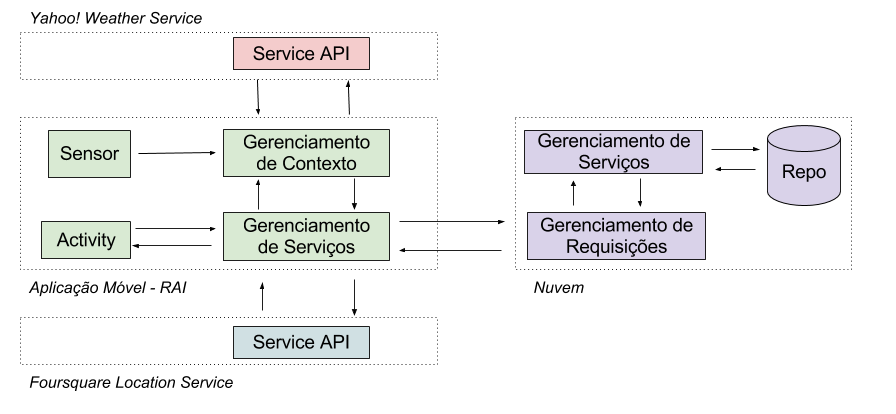
\includegraphics[width=\textwidth]{../figuras/arquitetura-rai.png}
	\caption{Arquitetura de sistema mostrando os componentes envolvidos e suas interações.}
	\label{fig:arquitetura-rai}
\end{figure}

\section{Especificação de Requisitos do Sistema}

\subsection{Requisitos Funcionais}
Os requisitos funcionais são:
\begin{itemize}
\item Cadastrar usuário;
\item Login de usuário
\item Buscar pontos de interesses mais próximos;
\item Ver condições climáticas;
\item Buscar sugestão de pontos de interesses utilizando filtro;
\item Buscar pontos de interesse mais próximos;
\item Buscar pontos de interesse por categoria, ou seja, utilizando filtro;
\item Ver detalhes de uma ponto de interesse (nome, posição no mapa, avaliação)
\item Avaliar item da recomendação.
\end{itemize}

\subsection{Requisitos Não-Funcionais}
Os requisitos não funcionais são:
\begin{itemize}
\item Dispositivo móvel equipado com sistema opercional \emph{Android} versão mínima $2.3.3$. Além disso o celular deve ser equipado com sensor de GPS e conectividade wireless (WiFi, GSM, 3G, 3G+ ou 4G);
\item O sistema deve ter uma interface intuitiva com o usuário, apresentando menus simples e diretos para facilitar a utilização da aplicação;
\item O sistema deve gerenciar da melhor forma possível o uso da bateria do dispositivo.
\end{itemize}

\section{Casos de Uso}
\subsection{Visão Geral}

\begin{figure}[htb]
\centering
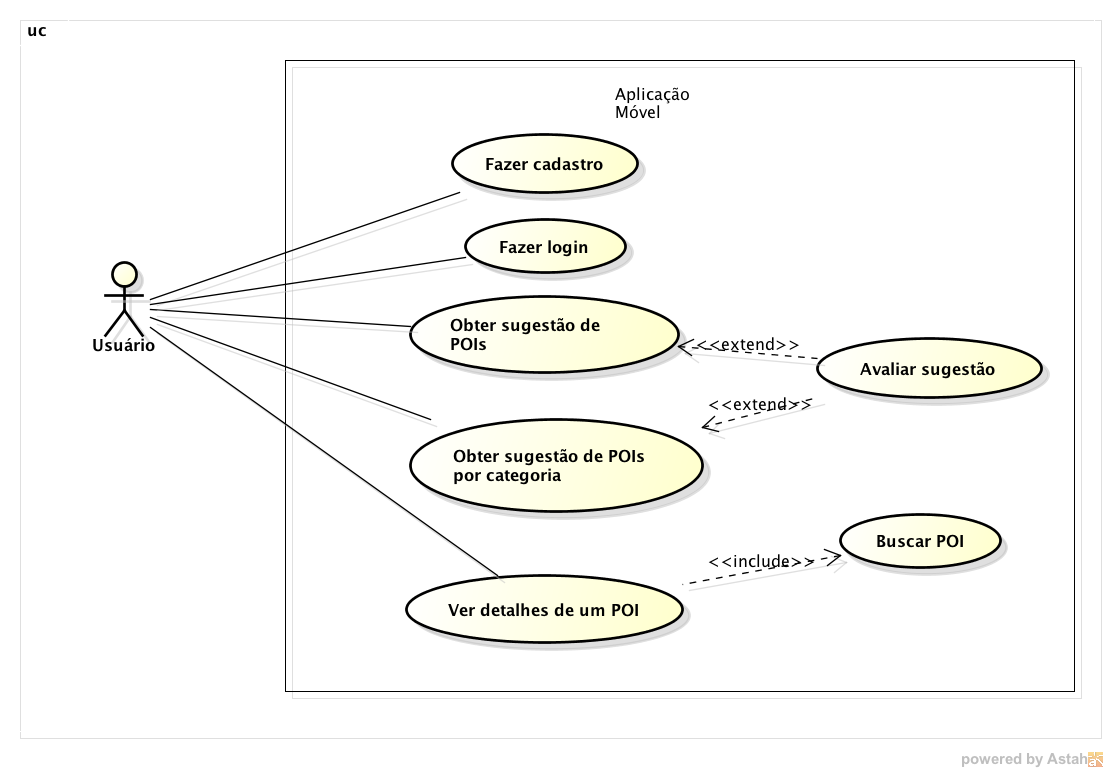
\includegraphics[scale=0.45]{../casos-de-usos/casos-de-usos-usuario-app.png}
\caption{Casos de usos para o ator \emph{usuário}.}
\label{fig:casos-de-usos-app-servidor}
\end{figure}

\begin{figure}[htb]
\centering
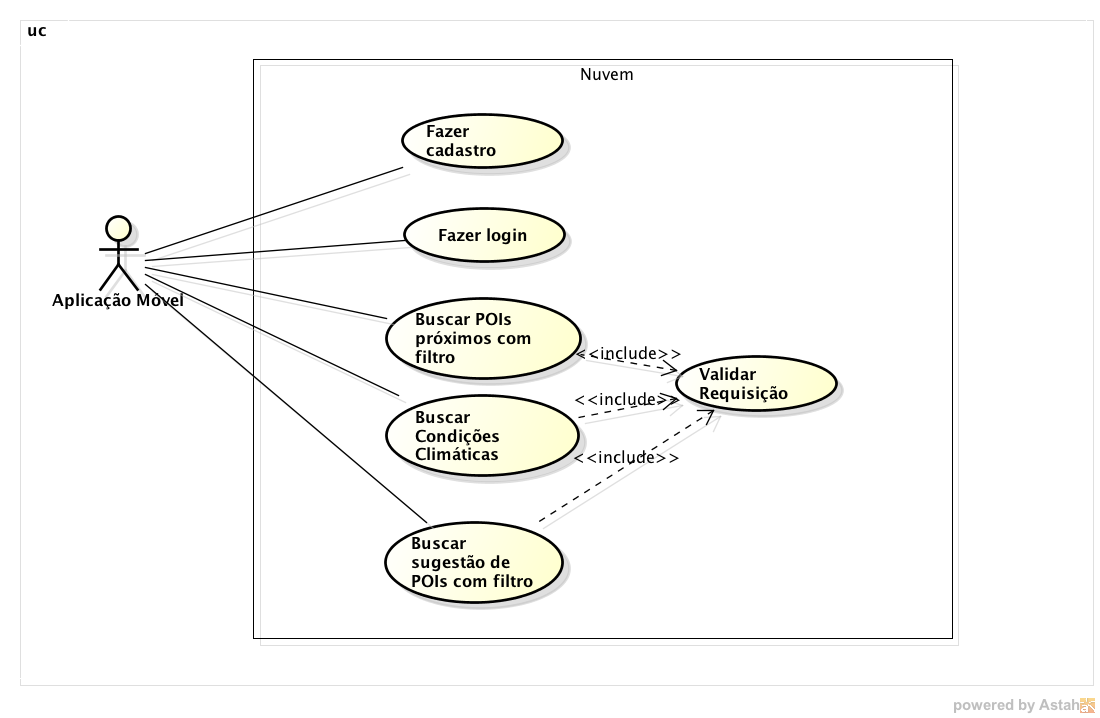
\includegraphics[scale=0.45]{../casos-de-usos/casos-de-usos-app-servidor.png}
\caption{Casos de usos para o ator \emph{aplicação móvel}.}
\label{fig:casos-de-usos-app-servidor}
\end{figure}

\subsection{Atores}
Os atores envolvidos no sistema são:
\begin{description}
\item \textbf{Usuário}. Usuário da aplicação móvel que busca informações ao seu redor bem como recomendações de pontos de interesses na cidade de Fortaleza;
\item \textbf{Aplicação Móvel}. A aplicação móvel é um ator para o consumo de serviços oferecidos pela nuvem.
\end{description}

\subsection{Casos de Usos}

Os casos de usos abaixo são referentes ao ator \textbf{usuário} da aplicação móvel.

\begin{uc}
\ucform
{RAI-UC}
{Fazer Cadastro}
{Usuário faz seu cadastro no sistema.}
{Essencial.}
{
\begin{itemize}
\item Fluxo principal:
	\begin{enumerate}
		\item O usuário seleciona a opção “Fazer cadastro” na tela inicial do sistema
		\item O sistema solicita as informações de usuário e senha
		\item O usuário preenche os dados e seleciona a opção “Cadastrar”
		\item O sistema cria a conta do novo usuário e exibe mesagem de sucesso
		\item O caso de uso se encerra
	\end{enumerate}
\end{itemize}
}
{Aplicação deve estar com acesso à Internet}
{A conta do novo usuária é criada}
\end{uc}

\begin{uc}
\ucform
{RAI-UC}
{Fazer login}
{Usuário faz login no sistema.}
{Essencial.}
{
\begin{itemize}
\item Fluxo principal:
	\begin{enumerate}
		\item O usuário insere \emph{username} e \emph{password}.
		\item O usuário preciona a opção ``Login''.
		\item O caso de uso se encerra.
	\end{enumerate}
\end{itemize}
}
{Aplicação deve estar com acesso à Internet}
{O usuário ``loga-se'' no sistema.}
\end{uc}

\begin{uc}
\ucform
{RAI-UC}
{Obter sugestão de pontos de interesse}
{Usuário solicita ao sistema uma lista com sugestões de com pontos de interesse.}
{Essencial}
{
\begin{itemize}
\item Fluxo principal:
	\begin{enumerate}
		\item O usuário seleciona a opção “Obter sugestão de locais” na tela inicial do sistema;
		\item O sistema exibe tela de seleção de categorias de pontos de interesse com a opção “Todos” previamente selecionada;
		\item O usuáiro seleciona a opção ``Confirmar'';
		\item O sistema obtém as informações de contexto do usuário e exibe uma lista de pontos de interesse sugeridos independemente de categoria;
		\item O caso de uso se encerra.
	\end{enumerate}
	\item Fluxo de exceção:
		\begin{enumerate}
			\item Aplicação não se comunidade com a nuvem
		\end{enumerate}
\end{itemize}
}
{Aplicação deve estar com acesso à Internet.}
{Sistema exibe lista de pontos de interesse sugeridos.}
\end{uc}

\begin{uc}
\ucform
{RAI-UC}
{Obter sugestão de pontos de interesse por categoria}
{Usuário solicita ao sistema uma lista com sugestões de com pontos de interesse de uma ou mais categorias.}
{Essencial}
{
\begin{itemize}
\item Fluxo principal:
	\begin{enumerate}
		\item O usuário seleciona a opção “Obter sugestão de locais” na tela inicial do sistema;
		\item O sistema exibe tela de seleção de categorias de pontos de interesse com a opção “Todos” previamente selecionada;
		\item O usuário seleciona uma ou mais categorias de pontos de interesse;
		\item O usuáiro seleciona a opção “Confirmar'';
		\item O sistema obtém as informações de contexto do usuário e exibe uma lista de pontos de interesse sugeridos de acordo com as categorias selecionadas pelo usuário.
	\end{enumerate}
\end{itemize}
}
{Aplicação deve estar com acesso à Internet.}
{Sistema exibe lista de pontos de interesse sugeridos.}

\end{uc}

\begin{uc}
\ucform
{RAI-UC}
{Ver detalhes de um ponto de interesse.}
{Usuário deseja ver os detalhes de um ponto de interesse.}
{Essencial}
{
\begin{itemize}
\item Fluxo principal:
	\begin{enumerate}
\item O usuário seleciona a opção “Buscar ponto de interesse” na tela inicial do sistema
\item O sistema solicita que o usuário informe o nome do ponto de interesse.
\item O usuário informa o nome do ponto de interesse e seleciona a opção “Buscar”.
\item O sistema exibe uma lista de pontos de interesse de acordo com o nome informado pelo usuário.
\item O usuário seleciona um dos pontos de interesse.
\item O sistema exibe os detalhes do ponto de interesse (nome, posição no mapa, avaliação)
\item O caso de uso se encerra.
	\end{enumerate}
\end{itemize}
}
{Aplicação deve estar com acesso à Internet.}
{ Sistema exibe os detalhes do ponto de interesse selecionado.}
\end{uc}

\begin{uc}
\ucform
{RAI-UC}
{Avaliar uma sugestão.}
{Usuário deseja avaliar uma sugestão de ponto de interesse feita pelo sistema.}
{Essencial}
{
\begin{itemize}
\item Fluxo principal:
	\begin{enumerate}
\item O usuário seleciona a opção ``Obter sugestão de locais'' na tela inicial do sistema
\item O sistema exibe tela de seleção de categorias de pontos de interesse com a opção “Todos” previamente selecionada.
\item O usuário mantém a opção ``Todos'' selecionada ou seleciona uma ou mais categorias de pontos de interesse.
\item O usuáiro seleciona a opção ``Confirmar''
\item O sistema obtém as informações de contexto do usuário e exibe uma lista de pontos de interesse sugeridos de acordo com os critérios do usuário.
\item O usuário seleciona um dos pontos de interesse.
\item O sistema exibe os detalhes do ponto de interesse (nome, posição no mapa, avaliação)
\item O usuário seleciona a opção ``Avaliar sugestão''
\item O sistema solicita a nota ao usuário
\item O usuário informa a nota (pode ser numérica ou no formato 5 estrelas) e seleciona a opção ``Confirmar''
\item O caso de uso se encerra.
	\end{enumerate}
\end{itemize}
}
{Aplicação deve estar com acesso à Internet.}
{Sistema salva a avaliação informada pelo usuário para a sugestão em questão.}
\end{uc}

Os casos de usos abaixo são referentes ao ator \textbf{aplicação móvel}.

\begin{uc}
\ucform
{RAI-UC}
{Cadastra usuário no sistema}

{Essencial}
{
\begin{itemize}
\item Fluxo principal:
\begin{enumerate}
\item Aplicação envia um \emph{username} e uma \emph{senha} de usuário para nuvem;
\item O caso de uso se encerra.
\end{enumerate}
\end{itemize}
}
{Aplicação deve está com acesso à Internet}
{Aplicação recebe confirmação de cadastro realizado com sucesso}
\end{uc}

\begin{uc}
\ucform
{RAI-UC}
{Fazer login}
{Aplicação móvel faz login no sistema.}
{Essencial.}
{
\begin{itemize}
\item Fluxo principal:
	\begin{enumerate}
		\item A aplicação móvel envia requisição com \emph{username} e \emph{password} para a nuvem.
		\item O caso de uso se encerra.
	\end{enumerate}
\end{itemize}
}
{Aplicação deve estar com acesso à Internet}
{A aplicação recebe confirmação de login válido.}
\end{uc}

\begin{uc}
\ucform
{RAI-UC}
{Buscar os POIs mais próximos}
{Buscar os POIs que estão mais próximos a uma dada posição espacial}
{Essencial}
{
\begin{itemize}
\item Fluxo principal:
\begin{enumerate}
\item Aplicação envia requisição de um usuáro com informação de contexto (posição espacial, tempo);
\item O caso de uso se encerra.
\end{enumerate}
\end{itemize}
}
{Aplicação deve está com acesso à Internet e está com sensor de posicionamento habilitado}
{Aplicação recebe uma lista de locais}
\end{uc}


\begin{uc}
\ucform
{RAI-UC}
{Buscar sugestão de POIs com filtro}
{Recomendar uma lista de POIs para o usuário considerando o contexto e um filtro (categoria dos POIs)}
{Essencial}
{
\begin{itemize}
\item Fluxo principal:
\begin{enumerate}
\item Aplicação envia requisição de um usuáro com informações de contexto e um filtro;
\item O caso de uso se encerra.
\end{enumerate}
\end{itemize}
}
{Aplicação deve está com acesso à Internet e está com sensor de posicionamento habilitado}
{Aplicação recebe uma lista de locais recomendados a serem visitados}
\end{uc}

%
\begin{uc}
\ucform
{RAI-UC}
{Buscar condições climáticas}
{Buscar condições climáticas de um dado local referente a um local na cidade}
{Essencial}
{
\begin{itemize}
\item Fluxo principal:
\begin{enumerate}
\item Aplicação envia requisição de um usuáro com informações de contexto (posição espacial, tempo);
\item O caso de uso se encerra.
\end{enumerate}
\end{itemize}
}
{Aplicação deve está com acesso à Internet e está com sensor de posicionamento habilitado}
{Aplicação recebe informações sobre as condições climáticas}
{}
\end{uc}

%
\begin{uc}
\ucform
{RAI-UC}
{Validar requisição}
{As requisicões feitas pela aplicação móvel é verificada}
{Essencial}
{
\begin{itemize}
\item Fluxo principal:
\begin{enumerate}
\item A aplicação envia requisição para a nuvem;
\item O sistema na nuvem valida requisição;
\item O caso de uso se encerra.
\end{enumerate}
\end{itemize}
}
{Aplicação deve está com acesso à Internet e está com sensor de posicionamento habilitado}
{Aplicação recebe informações sobre as condições climáticas}
{}
\end{uc}

%\section{Modelos de Sistemas}
%
%\section{Evolução de Sistema}

\end{document}